\documentclass[oneside]{article}
\usepackage{fancyhdr}
\usepackage{graphicx}
\pagestyle{fancy}
\title{Parallel Design Patterns II}
\author{B138813}
\date{February 2019}

\begin{document}
\lhead{Parallel Design Patterns II}
\rhead{B138813}

\maketitle
\section{Introduction}
We present our report for the second submission of the Parallel Design Patterns Coursework. We first discuss our implementation in Section~\ref{sec:imp}, and demonstrate its correctness in Section~\ref{sec:cor}. Although our implementation has some features similar to a framework, we were not able to succesfully seperate policy and mechanism to an adaquete extend. We will discuss this issue further in Section~\ref{sec:fur}.

\section{Implementation}\label{sec:imp}
We implemented our squirrel simulation in C++. We present a UML diagram of our implementation in Figure~\ref{fig:uml}. To maximise code re-use, we abstracted as much common functionality into the parent actor class as possible. The actor class holds methods such as \texttt{send\_msg()} and \texttt{msg\_recv()} which act as wrappers to MPI functions, whilst also providing extra functionality. For example, \texttt{msg\_recv()} returns a three item tuple, which contains:
\begin{itemize}
  \item A boolean, which indicates if the message was succesfully recieved.
  \item An integer, which indicates where the message was recived from.
  \item An integer, which is the message itself.
\end{itemize}
The semantics of the message integer are encoded into the \texttt{MSG} enum, which is shared by all actors. This standardisation makes it easy for the programmer to reason about messages, allowing them to dictate how a message if handled in each child class's main event loop. The function \texttt{send\_msg()} is simple convenience wrapper around \texttt{MPI\_Bsend()}.
\begin{figure}[h]
  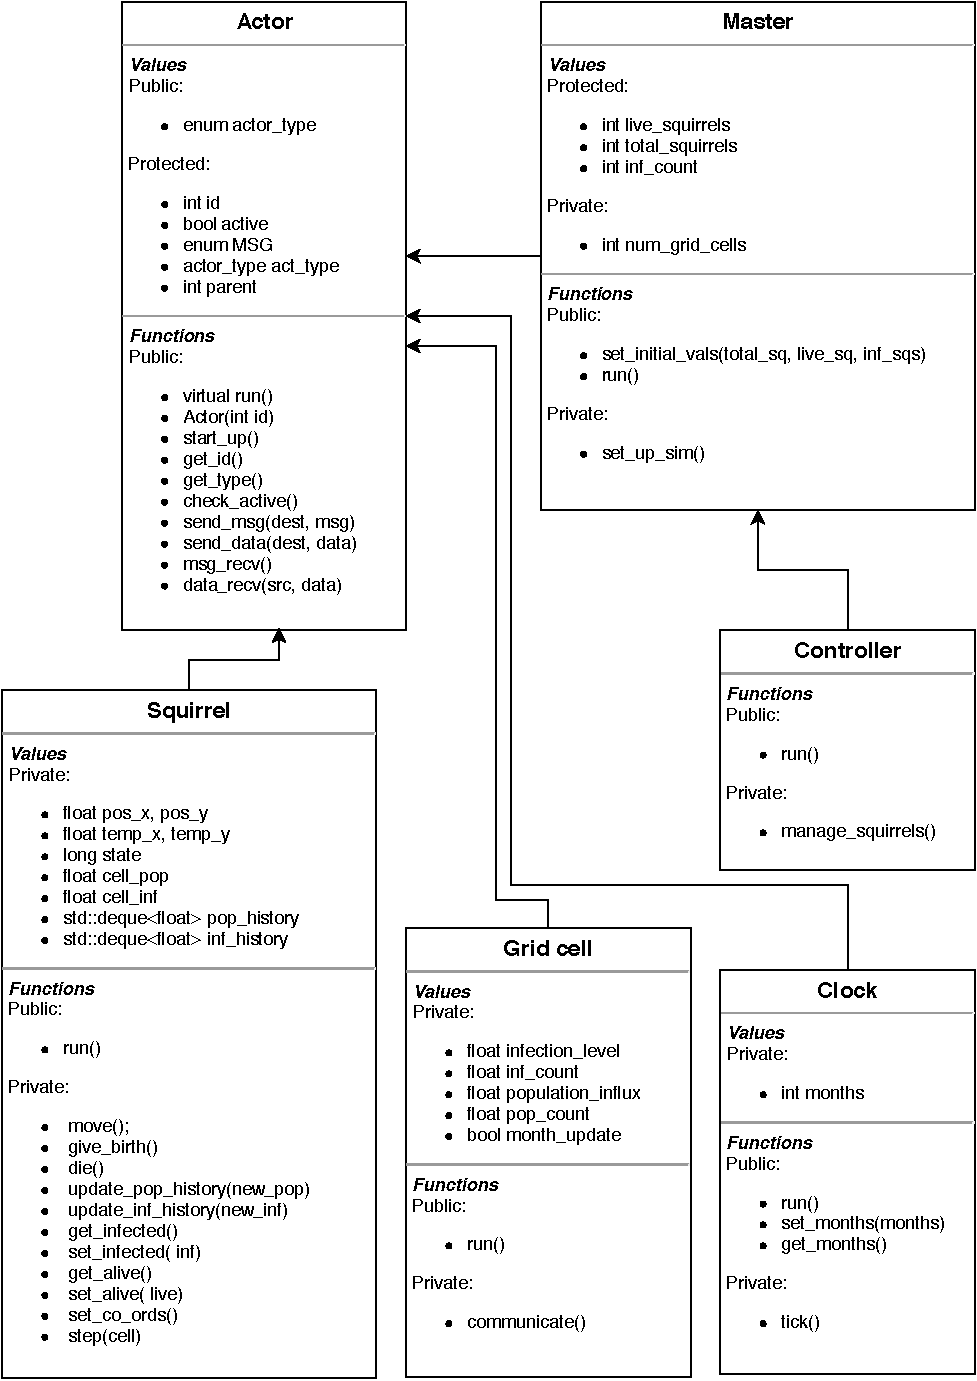
\includegraphics[width=\linewidth]{figures/pdp_uml}
  \caption{UML Diagram of the Program}
  \label{fig:uml}
\end{figure}
Each class inherits directly from the actor class, except for the controller, which is a child of the master class. We made this decision because the master and controller share most of their functionality and variables. Both classes need to know what the simulation's initial values, and share a function to implement this. If C++'s inheritance model did not allow both child and grandchild classes to implement their own versions their parent's virtual functions, this pattern would not be possible.

\section{Correctness}\label{sec:cor}

\section{Further Work}\label{sec:fur}

\end{document}
